\documentclass{beamer}
\usepackage[utf8]{inputenc}
\usepackage{graphicx}

% Remove navigation controls
\usenavigationsymbolstemplate{}

% Slide numbering
\setbeamertemplate{footline}[frame number]

\title{Integrity constraint checking of RDF bases using SPARQL}
\subtitle{
  A brief introduction to the subject of my training period
}
\author{
  Leandro Lovisolo
}
\date{September 11, 2015}
\institute{
  I.N.R.A. SupAgro \\
  Montpellier, France
}

\begin{document}

\begin{frame}
  \titlepage
\end{frame}

\begin{frame}
  \frametitle{Motivation}
  \framesubtitle{Problem statement}

  \pause

  \begin{itemize}
    \item We're trying to answer questions that require consulting heterogeneous data sources.

    \pause

    \begin{itemize}
      \item Literature with inconsistent, semi-structured data.

      \pause

      \item No standard naming convention.

      \pause

      \item No information about the reliability of the data sources.

      \pause

      \item Each data source has its specific browsing/querying mechanism (no common interface.)
    \end{itemize}
  \end{itemize}
\end{frame}

\begin{frame}
  \frametitle{Motivation}
  \framesubtitle{Example 1}

  \begin{itemize}
    \item Ligno-cellulosic biomass pre-treatment before enzymatic hydrolysis is an essential step to obtain good yields.

    \pause

    \item Several pre-treatment principles available, but \textbf{no clear criteria on how to choose the best one} taking into account environmental sustainability for a given biomass and biorefinery product (e.g. glucose.)
  \end{itemize}
\end{frame}

\begin{frame}
  \frametitle{Motivation}
  \framesubtitle{Example 2}

  \begin{itemize}
    \item TODO: Packaging example.
  \end{itemize}
\end{frame}

\begin{frame}
  \frametitle{Proposed solution}

  \begin{itemize}
    \item Represent scientific knowledge using ontologies using recommended standardized tools and languages for such purposes (semantic web technologies, RDF(S), OWL, etc.)

    \pause

    \item Develop an ontology and data management web application (e.g. the \textbf{@Web platform}) that makes it easy for scientists to introduce data from scientific publications into an ontology, execute queries against an ontology, etc.
  \end{itemize}
\end{frame}

\begin{frame}
  \frametitle{An example of a termino-ontological resource}
  \framesubtitle{Taken from the biorefinery domain}

  \begin{center}
    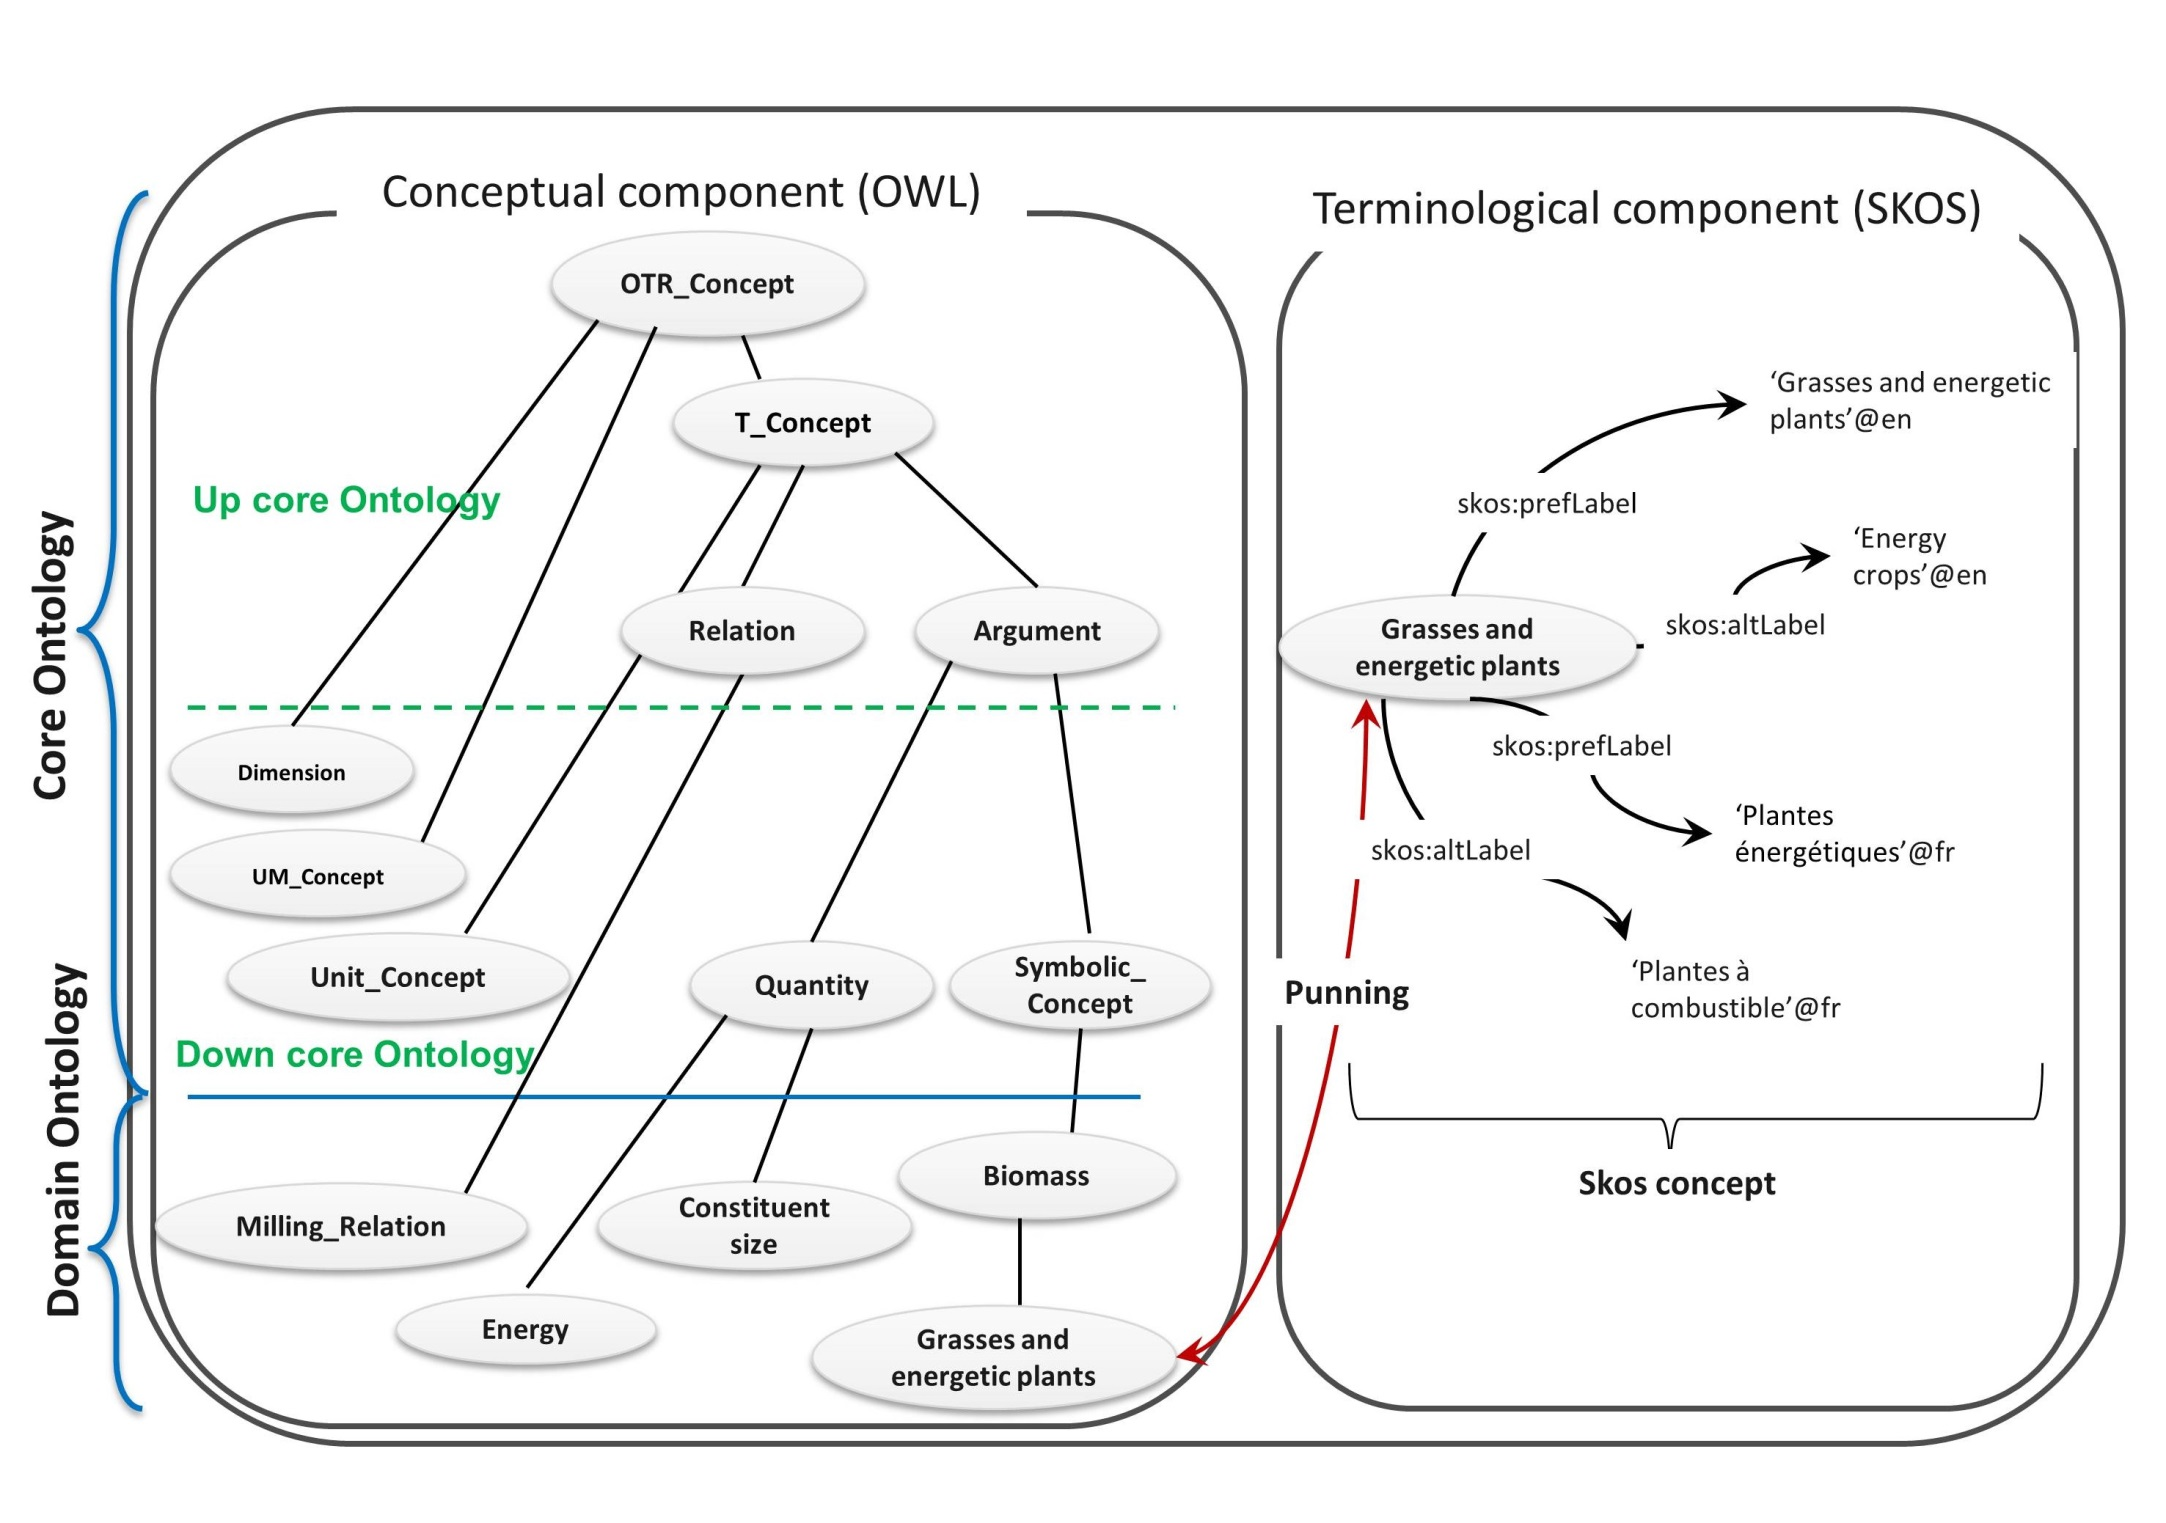
\includegraphics[width=10cm]{termino-ontological-resource.jpg}
  \end{center}
\end{frame}

\begin{frame}
  \frametitle{An example of a termino-ontological resource}
  \framesubtitle{Design goals}

  \begin{itemize}
    \item \textbf{Simple} so as to make the annotator's task easier.

    \pause

    \item \textbf{Generic} enough so that the approach can be applied to different, unrelated domains.

    \pause

    \begin{itemize}
      \item Proven in the domains of biorefinery and packaging selection.
    \end{itemize}
  \end{itemize}
\end{frame}

\begin{frame}
  \frametitle{A sample relation}
  \framesubtitle{Also from the biorefinery domain}

  \begin{center}
    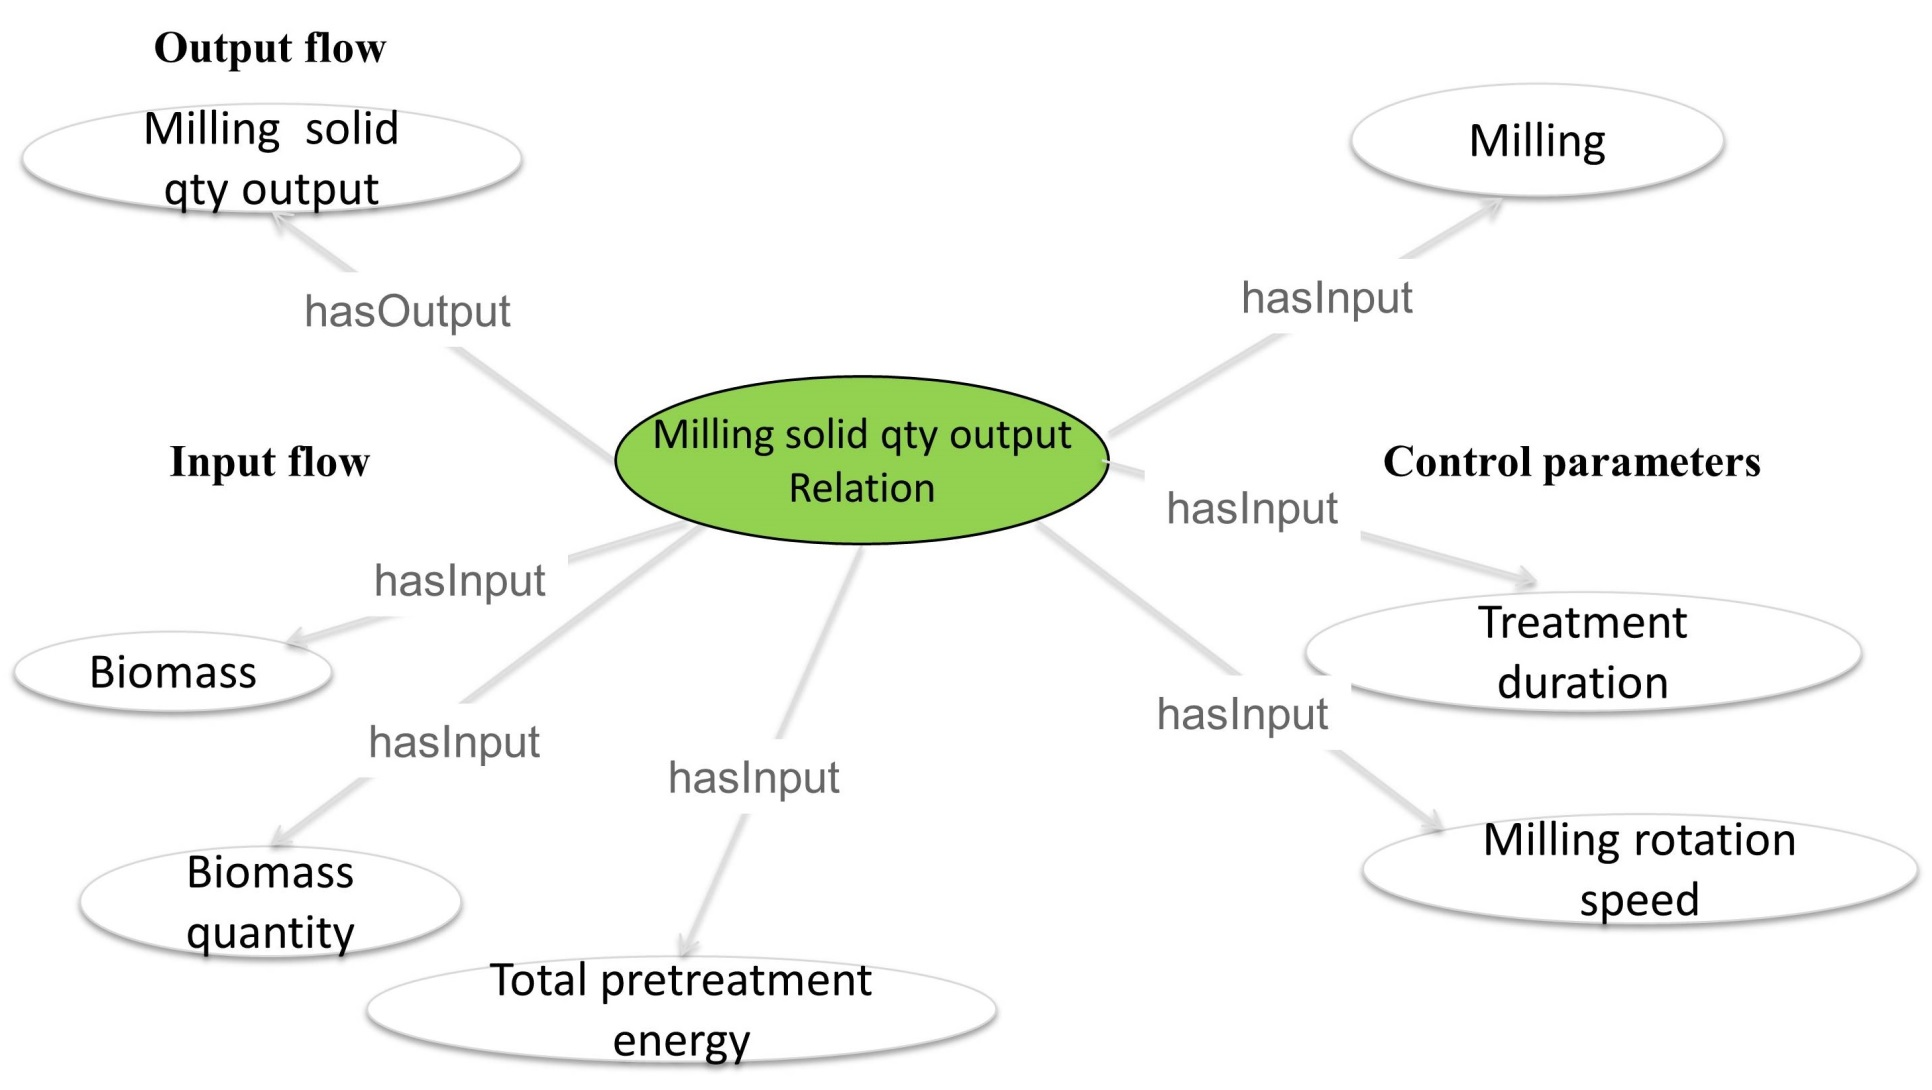
\includegraphics[width=10cm]{relation.jpg}
  \end{center}
\end{frame}

\begin{frame}
  \frametitle{The annotator's task}

  \begin{itemize}
    \item Given a scientific publication and a desired ontology, capture data from the publication using the appropriate concepts in the ontology.

    \pause

    \item Create and update concepts in the ontology as they're discovered during the annotation process (i.e. in an iterative fashion.)

    \pause

  \item Write and edit \textbf{guidelines} associated to each concept explaining when and how a concept should be used.
  \end{itemize}
\end{frame}

\begin{frame}
  \begin{center}
    \Huge{Q\&A}
  \end{center}
\end{frame}

\begin{frame}
  \begin{center}
    \Huge{Thanks!}
  \end{center}
\end{frame}

\end{document}
